\chapter{Sprachsynthese}


\begin{figure}[htbp]
\begin{center}
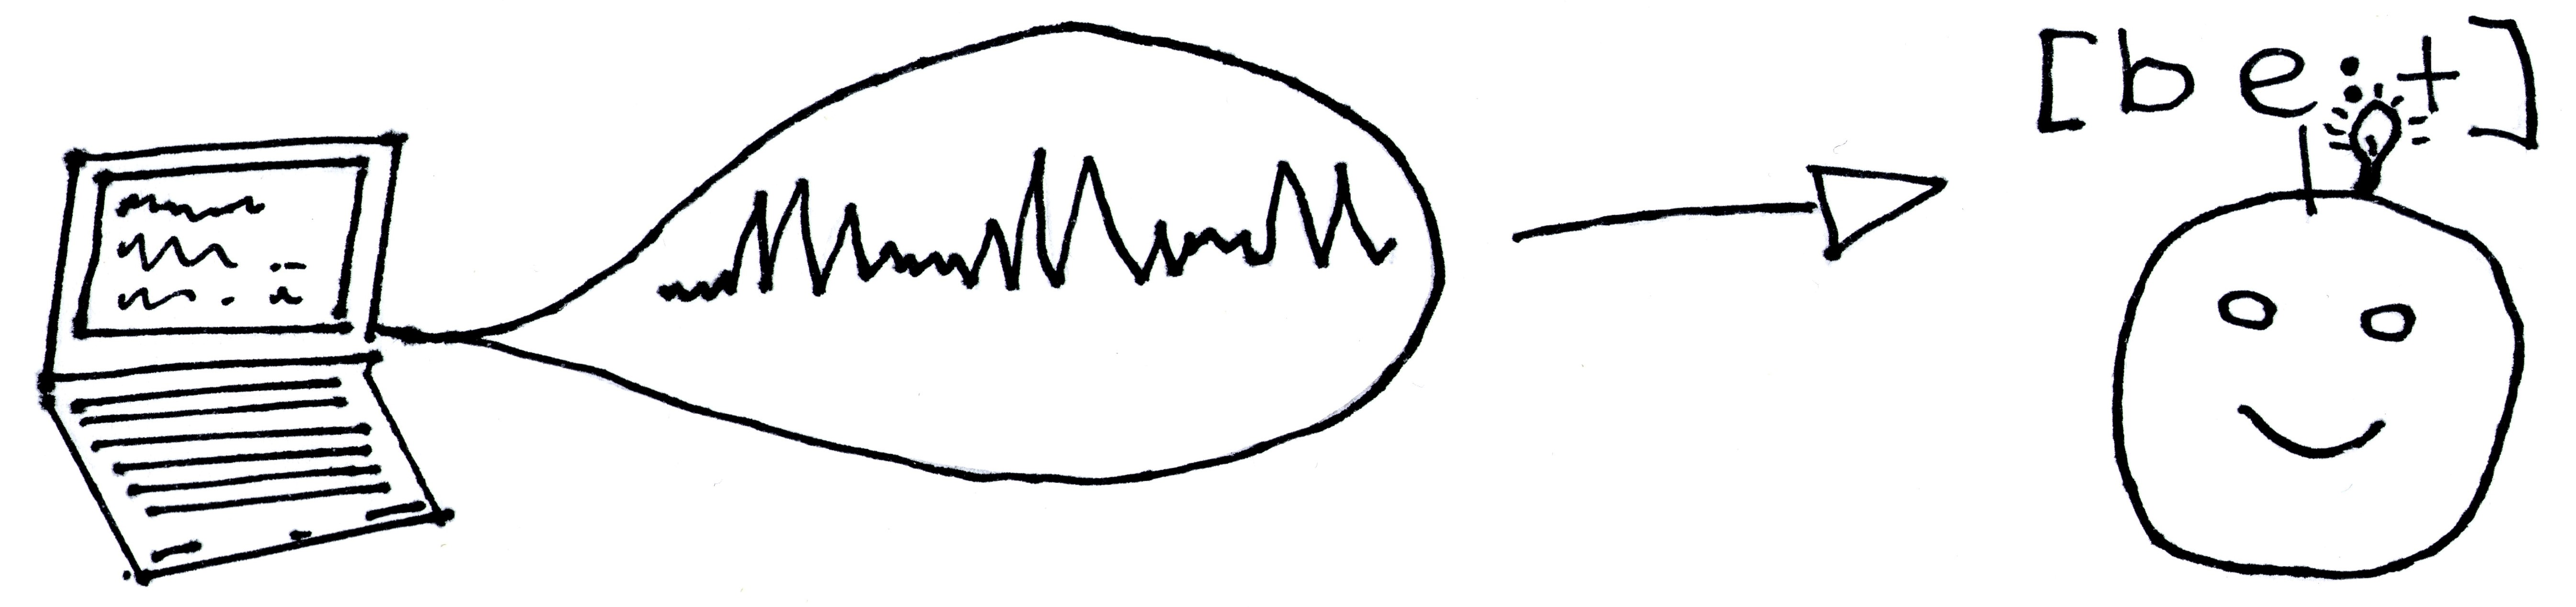
\includegraphics[width=\textwidth]{grafiken/sprachsynthese/synthese.jpg}
\label{ts}
\end{center}
\end{figure}

\section{Stichworte zum Vortrag \em{Sprachsynthese}}

Text-to-Speech, Concept-to-Speech, Formantsynthese, artikulatorische Synthese, konkatenative Synthese, Textnormalisierung, Graphem-Phonem-Konvertierung



\section{Literatur}


\emph{Eine gute Einführung findet sich in Kapitel 8:}\\
Jurafsky, Dan \& Martin, James H. (2000): Speech \& language processing. Pearson Education India

\emph{Kapitel 3 in:}\\
Pfister B., Kaufmann T. (2008): Sprachverarbeitung - Grundlagen und 
	Methoden der Sprachsynthese und Spracherkennung. 
	Springer-Verlag Berlin Heidelberg.


\renewcommand\refname{\vskip -1cm}
\bibliography{synthese}{}
\bibliographystyle{plain}

%%%%%%%%%%%%%%%%%%%%%%%%%%%%%%
%%%%%%%%%%%%%%%%%%%%%%%%%%%%%%
